\documentclass[tikz,border=12pt]{standalone}
\usepackage{amsmath,amssymb}
\usetikzlibrary{calc,arrows.meta}

\begin{document}
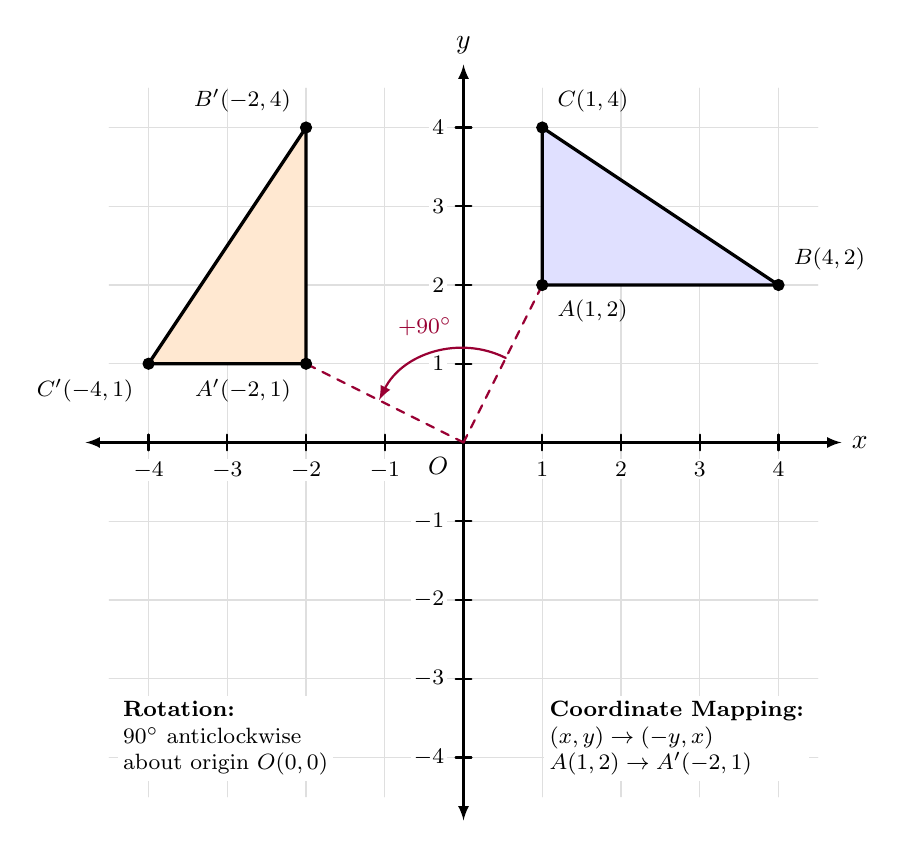
\begin{tikzpicture}[>=latex, line cap=round, line join=round]
  % Grid
  \draw[step=1cm, gray!25, thin] (-4.5, -4.5) grid (4.5, 4.5);

  % Axes
  \draw[thick, <->] (-4.8, 0) -- (4.8, 0) node[right, font=\normalsize] {$x$};
  \draw[thick, <->] (0, -4.8) -- (0, 4.8) node[above, font=\normalsize] {$y$};

  % Origin
  \node[below left=2pt, font=\small] at (0, 0) {$O$};

  % Integer ticks with opaque backgrounds
  \foreach \x in {-4,-3,-2,-1,1,2,3,4} {
    \draw[thick] (\x, 0.1) -- (\x, -0.1);
    \node[below=3pt, font=\footnotesize, fill=white, inner sep=1pt] at (\x, -0.1) {$\x$};
  }
  \foreach \y in {-4,-3,-2,-1,1,2,3,4} {
    \draw[thick] (0.1, \y) -- (-0.1, \y);
    \node[left=3pt, font=\footnotesize, fill=white, inner sep=1pt] at (-0.1, \y) {$\y$};
  }

  % Coordinates
  % Object triangle ABC (Quadrant I)
  \coordinate (A) at (1, 2);
  \coordinate (B) at (4, 2);
  \coordinate (C) at (1, 4);

  % Image triangle A'B'C' (Quadrant II) under 90 deg anticlockwise rotation (x, y) -> (-y, x)
  \coordinate (A1) at (-2, 1);
  \coordinate (B1) at (-2, 4);
  \coordinate (C1) at (-4, 1);

  % Radial guide lines from Origin to A and A'
  \draw[thick, dashed, purple!80!black] (0,0) -- (A);
  \draw[thick, dashed, purple!80!black] (0,0) -- (A1);

  % 90 deg rotation arc between OA and OA'
  % angle of A: atan(2/1) = 63.435 deg; angle of A1: 180 - atan(1/2) = 153.435 deg
  \draw[thick, ->, purple!80!black] (63.435:1.2) arc (63.435:153.435:1.2);
  \node[font=\footnotesize\bfseries, purple!80!black, fill=white, inner sep=1pt] at (108.435:1.55) {$+90^\circ$};

  % Object triangle ABC
  \draw[very thick, fill=blue!12] (A) -- (B) -- (C) -- cycle;
  \filldraw[black] (A) circle (2pt) node[below right=2pt, font=\footnotesize\bfseries] {$A(1,2)$};
  \filldraw[black] (B) circle (2pt) node[above right=2pt, font=\footnotesize\bfseries] {$B(4,2)$};
  \filldraw[black] (C) circle (2pt) node[above right=2pt, font=\footnotesize\bfseries] {$C(1,4)$};

  % Image triangle A'B'C'
  \draw[very thick, fill=orange!18] (A1) -- (B1) -- (C1) -- cycle;
  \filldraw[black] (A1) circle (2pt) node[below left=2pt, font=\footnotesize\bfseries] {$A'(-2,1)$};
  \filldraw[black] (B1) circle (2pt) node[above left=2pt, font=\footnotesize\bfseries] {$B'(-2,4)$};
  \filldraw[black] (C1) circle (2pt) node[below left=2pt, font=\footnotesize\bfseries] {$C'(-4,1)$};

  % Rule Annotation in Quadrants III and IV
  \node[align=left, font=\footnotesize, fill=white, inner sep=2pt, anchor=south west] at (-4.4, -4.3) {\textbf{Rotation:}\\ $90^\circ$ anticlockwise\\ about origin $O(0,0)$};
  \node[align=left, font=\footnotesize, fill=white, inner sep=2pt, anchor=south east] at (4.4, -4.3) {\textbf{Coordinate Mapping:}\\ $(x, y) \to (-y, x)$\\ $A(1,2) \to A'(-2,1)$};

\end{tikzpicture}
\end{document}
